\chapter{Matrices}
Let us consider a linear combination of vectors
\[
x_1\cdot\colvec{3}{u_1}{\vdots}{u_n}+x_2\cdot\colvec{3}{v_1}{\vdots}{v_n}+x_3\cdot\colvec{3}{w_1}{\vdots}{w_n} = \colvec{3}{b_1}{\vdots}{b_n}
\]
This can be written using matrices in the following way:
\[
\begin{pmatrix}
u_1 & v_1 & w_1\\
\vdots & \vdots & \vdots\\
u_n & v_n & w_n
\end{pmatrix}\cdot \colvec{3}{x_1}{x_2}{x_3} =
\colvec{3}{b_1}{\vdots}{b_n}
\]
In matrix-vector multiplication, we take dot products of rows of matrices times the vector.
\begin{example}
\begin{enumerate}
\item \[
\begin{pmatrix}
1 & 0 & -1\\
3 & 1 & 2\\
1 & -1 & 5\\
\end{pmatrix}
\cdot
\begin{pmatrix}
1\\
0\\
1\\
\end{pmatrix}
 = 
\begin{pmatrix} 
 1 \cdot 1 + 0 \cdot 0 + (-1) \cdot 1\\ 
 3 \cdot 1 + 1 \cdot 0 + 2 \cdot 1\\ 
 1 \cdot 1 + (-1) \cdot 0 + 5 \cdot 1\\
\end{pmatrix} 
 = 
 \begin{pmatrix} 
 0\\ 
 5\\ 
 6\\
\end{pmatrix}
\]
\begin{notation}
Matrices are usually written with capital letters, i.e. $A,B,c,\dots$\\

$A$ is an $n$ by $m$ matrix, $A\in\R^{n,m}$	 if it has $n$ rows and $m$ columns.\\

The element of matrix $A$ located in row $i$ and column $j$ is written as $a_{ij}$ or $(A)_{ij}$.
\end{notation}
\item 
\begin{align*}
A &= \begin{pmatrix}
-1 & 2 & 3\\
0 & 1 & 0
\end{pmatrix}, \ul{x} = \colvec{3}{1}{1}{1}\\
A\cdot\ul{x} &=\begin{pmatrix}
-1 & 2 & 3\\
0 & 1 & 0\\
\end{pmatrix}
\cdot
\begin{pmatrix}
1\\
1\\
1\\
\end{pmatrix}
 \\ &= 
\begin{pmatrix} 
 (-1) \cdot 1 + 2 \cdot 1 + 3 \cdot 1\\ 
 0 \cdot 1 + 1 \cdot 1 + 0 \cdot 1\\
\end{pmatrix} 
 = 
 \begin{pmatrix} 
 4\\ 
 1\\
\end{pmatrix}
\end{align*}
For the product of matrix $A$ with vector $\ul{x}$ to exist, matrix $A$ should have the same number of columns as vector $\ul{x}$ components.
\end{enumerate}
\end{example}

\section{Matrix Operations}
\begin{definition}
Let us consider matrices $A\in\R^{n,m}$ and $B\in\R^{n,m}$ where $n=$ rows, $m=$ columns. Matrix $C\in\R^{n,m}$ is a sum of $A$ and $B, C=A+B$ if $C_{ij} = A_{ij}+B_{ij}$ for all $i=1,\dots,n$, $j=1,\dots,m$
\end{definition}
\begin{example}
\[
A = \begin{pmatrix}
1 & 2\\
3 & 4\\
5 & 5
\end{pmatrix}, B = \begin{pmatrix}
-1 & 0\\
0 & -1\\
-1 & 0
\end{pmatrix}, C = A+B = \begin{pmatrix}
0 & 2\\
3 & 3\\
4 & 6
\end{pmatrix}
\]	
\end{example}
\begin{definition}
A product of a scalar $\alpha$ and a matrix $A\in\R^{n,m}$ is defined as $\left( \alpha A\right)_{ij} = \alpha\cdot A_{ij}$, $\forall i=1,\dots,n; j=1,\dots,m$.
\end{definition}
\begin{example}
\[\alpha = 3,A = \begin{pmatrix}
0 & 0 & 1\\
2 & 3 & 5	
\end{pmatrix}\Rightarrow \alpha\cdot A = \begin{pmatrix}
0 & 0 & 3\\
6 & 9 & 15
\end{pmatrix}
\]	
\end{example}
\begin{properties}
\begin{itemize}
\item $A\in\R^{n,m}$ and $B\in\R^{n,m}$: $A+B = B+A$\\
\ul{Proof:} 
\[
\begin{cases}
\left( A+B \right)_{ij} = A_{ij}+B_{ij}\\
\left( B+A \right)_{ij} = B_{ij}+A_{ij}
\end{cases}
\]
\item $A,B,C\in\R^{n,m}$: $(A+B)+C = A+(B+C)$
\item $\alpha\cdot (A+B) = \alpha A+\alpha B$ for $\forall \alpha\in\R, A,B\in\R^{n,m}$
\end{itemize}
	
\end{properties}

\section{Matrix - Matrix multiplication}
\begin{definition}
Let us consider matrix $A\in\R^{n,m}$ and $A\in\R^{m,l}$. Then $C = A\cdot B$ is an $n$ by $l$ matrix, $C\in\R^{n,l}$ such that 
\[
C_{ij} = \sum\limits^{n}_{k=1}a_{ik}b_{kj}
\]
\end{definition}
\begin{example}
\begin{enumerate}
\item \begin{align*}
A&= \begin{pmatrix}
1 & 2\\
0 & 1\\
3 & 4
\end{pmatrix}\in\R^{3,2}, B = \begin{pmatrix}
1 & 2 & 0 & 1\\
-1 & 1 & 1 & 0
\end{pmatrix}\in\R^{1,4}\\
C &= A\cdot B\in\R^{3,4}\\
&= \begin{pmatrix}
1 & 2\\
0 & 1\\
3 & 4
\end{pmatrix}\cdot \begin{pmatrix}
1 & 2 & 0 & 1\\
-1 & 1 & 1 & 0
\end{pmatrix} = \begin{pmatrix}
-1 & 4 & 2 & 1\\
-1 & 1 & 1 & 0\\
-1 & 10 & 4 & 3
\end{pmatrix}
\end{align*}
\item 
\[
A = \begin{pmatrix}
1 & 2 \\ 
0 & 1\\
3 & 4
\end{pmatrix}, B = \begin{pmatrix}
1 & 1 & 1\\
0 & 0 & 0\\
2 & 2 & 2
\end{pmatrix}; AB = \text{ Not defined}
\]
\end{enumerate}
\end{example}

\begin{properties}
\begin{enumerate}
\item $AB$ is  not always equal to $BA$. (most often, is the case). 
\begin{align*}
A &= \begin{pmatrix}
1 & 0\\
0 & 0
\end{pmatrix}, B = \begin{pmatrix}
0 & 1 \\
0 & 0
\end{pmatrix}\\
AB &= \begin{pmatrix}
0 & 1 \\
0 & 0
\end{pmatrix}, BA = \begin{pmatrix}
0 & 0 \\
0 & 0
\end{pmatrix}
\end{align*}
\item $C(A+B) = CA + CB$
\item $(A+B)C = AC+BC$
\item $\alpha (AB) = A(\alpha B)$, $A\in\R^{n,m}$, $B\in\R^{m,l}$. Proof:
\[
\left( \alpha(AB)\right)_{ij} = \alpha\sum\limits^{m}_{k=1} a_{ik}b_{kj} = \sum\limits^{m}_{k=1} a_{ik}(\alpha b_{kj}) = A(\alpha B)
\]
\item $(AB)C = A(BC)$
\end{enumerate}
\end{properties}

\begin{theorem}
Let us consider matrices $A\in\R^{n,n}$ and $B\in\R^{n,n}$, such that $A^{-1}$ and $B^{-1}$ exist. Then,
\[
(AB)^{-1} = B^{-1}\cdot A^{-1}
\]
\end{theorem}
\begin{proof}
\[
\begin{rcases*}
(AB)(B^{-1} A^{-1}) = I\\
(B^{-1} A^{-1})(AB) = I
\end{rcases*}\text{ Prove this}
\]
\begin{align*}
(AB)(B^{-1} A^{-1}) &= A\underbrace{BB^{-1}}_{I} A^{-1} = A\cdot I \cdot A^{-1} = I\\
(B^{-1} A^{-1})(AB) &= B^{-1}\underbrace{A^{-1}A}_{I} B =  \cdot B^{-1} \cdot I \cdot B= I\\
\end{align*}
$\Rightarrow$ According to the definition $B^{-1} A^{-1}$ is the inverse of $AB$
\end{proof}

\begin{lemma}
$A,B,C\in\R^{n,n}, \exists A^{-1},\exists B^{-1},\exists C^{-1}$ 
\[
(ABC)^{-1} = C^{-1}B^{-1}A^{-1}
\]
\end{lemma}

\begin{theorem}
Let us consider $A\in\R^{n,n}$. Let us consider that $B\in\R^{n,n}$ and $C\in\R^{n,n}$ are both inverses of $A$.Then $B=C$. (The inverse is unique)
\end{theorem}

\begin{proof}
\begin{center}
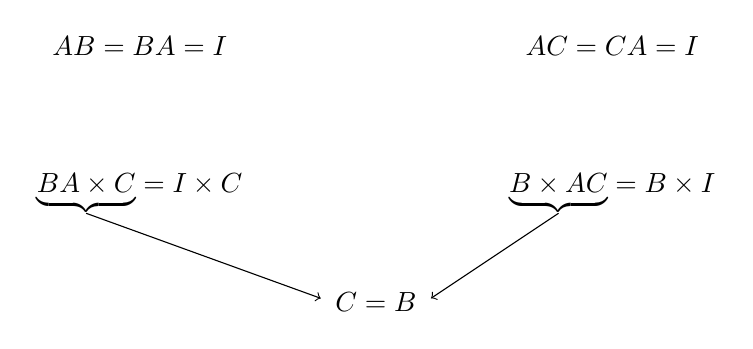
\begin{tikzpicture}
\draw(3,3) node[anchor=center]{$AC=CA=I$};
\draw(-3,3) node[anchor=center]{$AB=BA=I$};
\draw(-3,1) node[anchor=center]{$\underbrace{BA\times C}_{}=I\times C$};
\draw(3,1) node[anchor=center]{$\underbrace{B\times AC}_{}=B\times I$};
\draw[->] (2.32,0.88) --  (0.7,-0.2);
\draw[->,bend left=45] (-3.68,0.88) --  (-0.7,-0.2);
\draw(0,0) node[anchor=north]{$\ul{\ul{C=B}}$};
\end{tikzpicture}
\end{center}
\end{proof}

\section{Linear system of equations}
Let us consider the following system of equations
\[
\begin{cases}
2x_1+2x_2+4x_3 = 2\\
x_2+2x_3 = 3\\
4x_3 = -1
\end{cases}
\]
Find $x_1,x_2,x_3$. We can write this system in matrix form.
\[
A = \begin{pmatrix}
2 & 2 & 4\\
0 & 1 & 2\\
0 & 0 & 4
\end{pmatrix} \in\R^{3,3}, \ul{x} = \colvec{3}{x_1}{x_2}{x_3}, \ul{b} = \colvec{3}{2}{3}{-1} \Rightarrow A\ul{x} = \ul{b}
\]
$A$ is an upper triangular matrix. We can use backward substitution to find the solution:
\begin{enumerate}
\item $x_3 = -\frac{1}{4} = \frac{b_3}{a_{33}}$
\item $x_2 = \frac{3-2x_3}{1} = \frac{3-2\cdot \left( -\frac{1}{4}\right)}{1} = 3.5 = \frac{b_2-a_{33}\cdot x_3}{a_{22}}$
\item $x_1 = \frac{2-4x_3-2x_2}{2} = -2 = \frac{b_1-a_{13}x_3-a_{12}x_2}{a_{11}}$
\end{enumerate}
In general, if $A\in\R^{n,n}$ is an upper triangular with $a_{ii}\not=0, i=1,\dots,n$ then the backward substitution works as:
\begin{enumerate}
\item $x_n = \frac{b_n}{a_{nn}}$
\item $x_{n-1} = \frac{b_{n-1}-a_{n-1\hspace{1mm}n}x_n}{a_{n-1\hspace{1mm}n-1}}\hspace{5mm}\dots\hspace{5mm}x_i=$\todo{Cannot understand last calculation, page 12, LinearAlgebraNotes\_1}
\end{enumerate}

\section{Inverse Matrix}
\begin{definition}
Let us consider a matrix $A\in\R^{n,n}$ (square matrix). Matrix $B\in\R^{n,n}$ is called an inverse of $A$, if 
\[
A\cdot B = I\text{ \Large{AND} }B\cdot A = I
\]
(Both conditions are vital)
\end{definition}

\begin{notation}
Usually, the inverse of $A$ is written as $A^{-1}$
\end{notation}

\begin{note}
Not all matrices have an inverse! In most cases, it is quite difficult to find an inverse matrix. But in some cases, the inverse is easy to find.	
\end{note}
\begin{example}
\[
A = {\begin{pmatrix}
{{a_{11}}}&0& \ldots &0\\
0&{{a_{22}}}&{}& \vdots \\
 \vdots &{}& \ddots &0\\
0& \ldots &0&{{a_{nn}}}
\end{pmatrix}},a_{ii}\not=0,\forall i=1,\dots,n
\]	
Then

\begin{align*}
A &={\begin{pmatrix}
{a_{11}^{ - 1}}&0& \ldots &0\\
0&{a_{22}^{ - 1}}&{}& \vdots \\
 \vdots &{}& \ddots &0\\
0& \ldots &0&{a_{nn}^{ - 1}}
\end{pmatrix}}\\
A\cdot A^{-1} &= {\begin{pmatrix}
{{a_{11}}}&0& \ldots &0\\
0&{{a_{22}}}&{}& \vdots \\
 \vdots &{}& \ddots &0\\
0& \ldots &0&{{a_{nn}}}
\end{pmatrix}}	\cdot {\begin{pmatrix}
{a_{11}^{ - 1}}&0& \ldots &0\\
0&{a_{22}^{ - 1}}&{}& \vdots \\
 \vdots &{}& \ddots &0\\
0& \ldots &0&{a_{nn}^{ - 1}}
\end{pmatrix}}\\
 &= \left( {\begin{array}{*{20}{c}}
1&0& \ldots &0\\
0&1&{}& \vdots \\
 \vdots &{}& \ddots &0\\
0& \ldots &0&1
\end{array}} \right)\\
A\cdot A^{-1} &= I
\end{align*}	
\end{example}

\section{Special Matrices}
\begin{itemize}
\item Let us consider $A\in\R^{n,m}$ matrix. $A$ is called the zero matrix if all $a_{ij} = 0$, $\forall i=1,\dots,n;j=1,\dots,n$
\item $D\in\R^{n,n}$ - square matrix is called diagonal matrix, if $d_{ij} = 0$ and if $i\not=j$
\item Identity matrix: 
\[I\in\R^{n,n}, I=\begin{pmatrix}
1 & \dots & 0\\
\vdots & \ddots & \vdots\\
0 & \dots & 1
\end{pmatrix}
\]
\item $L\in\R^{n,n}$ - lower triangular matrix, if 
\[
l_{ij}=0, \forall i<j, L = \begin{pmatrix}
* & \dots & 0\\
\vdots & \ddots & \vdots\\
* & \dots & *
\end{pmatrix}
\]
\item $U\in\R^{n,n}$ - upper triangular matrix, if 
\[
u_{ij}=0, \forall i>j, L = \begin{pmatrix}
* & \dots & *\\
\vdots & \ddots & \vdots\\
0 & \dots & *
\end{pmatrix}
\]
\end{itemize}
\begin{remark}
If $A,B\in\R^{n,n}$ are both upper (lower) triangular matrices, then $C=A\cdot B$ is an upper triangular (lower).\\
\end{remark}

If $A$ is lower triangular, $A\in\R^{n,n}, a_{ii}\not = 0,i=1,\dots,n$ then we can use forward substitution, i.e.:
\begin{align*}
x_1 &= \frac{b_1}{a_{11}}	\\
&\vdots\\
x_i &= \frac{b_i-a_{i1}x_1-\dots-a_{ii-1}x_{i-1}}{a_{ii}}\hspace{5mm} \forall i = 2,\dots,n
\end{align*}
\section{Elementary Transition Matrices}
Let us consider matrix 
\[
A = \begin{pmatrix}
1 & 0 & -1 & 2\\
3 & 4 & 5 & 7\\
2 & -1 & 0 & 0\\
-1 & 3 & 5 & -1
\end{pmatrix}
\]
and matrix 
\[
I_{21} = \begin{pmatrix}
0 & 0 & 0 & 0\\
1 & 0 & 0 & 0\\
0 & 0 & 0 & 0\\
0 & 0 & 0 & 0
\end{pmatrix}
\]
Then
\[
I_{21}\cdot A = \begin{pmatrix}
0 & 0 & 0 & 0\\
1 & 0 & 0 & 0\\
0 & 0 & 0 & 0\\
0 & 0 & 0 & 0
\end{pmatrix}\cdot \begin{pmatrix}
1 & 0 & -1 & 2\\
3 & 4 & 5 & 7\\
2 & -1 & 0 & 0\\
-1 & 3 & 5 & -1
\end{pmatrix} = \begin{pmatrix}
0 & 0 & 0 & 0\\
1 & 0 & -1 & 2\\
0 & 0 & 0 & 0\\
0 & 0 & 0 & 0
\end{pmatrix}
\]
also
\[
A \cdot I_{21} = \begin{pmatrix}
1 & 0 & -1 & 2\\
3 & 4 & 5 & 7\\
2 & -1 & 0 & 0\\
-1 & 3 & 5 & -1
\end{pmatrix}\cdot\begin{pmatrix}
0 & 0 & 0 & 0\\
1 & 0 & 0 & 0\\
0 & 0 & 0 & 0\\
0 & 0 & 0 & 0
\end{pmatrix} = \begin{pmatrix}
0 & 0 & 0 & 0\\
4 & 0 & 0 & 0\\
-1 & 0 & 0 & 0\\
3 & 0 & 0 & 0
\end{pmatrix}
\]
\begin{definition}
We can define the elementary transition matrix $I_{pq}\in\R^{n,n}$
\[
\left( I_{pq}\right) = \begin{cases}
1 & i=p,q=j\\
0 & \text{otherwise}
\end{cases}
\]
If we take a matrix $A\in\R^{n,n}$ then when calculating $I_{pq}$ we take row $q$ of $A$, put it into row $p$, replace everything else with 0.\\

We can also define:
\begin{align*}
E_{pq}(l) &= I + l\cdot I_{pq}, l\in\R\text{ - scalar}\\
E_{pq}(l)\cdot A &= (I+lI_{pq})\cdot A = A + l\cdot I_{pq}A
\end{align*}
We take row $q$ of $A$, multiply it by $l$, add it to row $p$ of $A$
\[
E^{-1}_{pq}(l) = E_{pq}(-l)
\]
\end{definition}
If we have vector $\ul{b}\in\R^n$, then $I_{pq}\ul{b}$ - we take component $q$ of $\ul{b}$, put it into component $p$, replace everything else with zeros. 
\[
E_{pq}(l)\ul{b}\text{ - same as for matrices}
\]


